\documentclass{article}

\usepackage{geometry}
\geometry{left=2.5cm,right=2.5cm,top=2.5cm,bottom=2.5cm}

\pagenumbering{gobble}

\usepackage{hyperref}
\usepackage[none]{hyphenat}

\usepackage{graphicx}

\title{Haptic Object Exploration}
\date{}


\begin{document}


\maketitle % Print the title

\section*{Classification by EPs}

\subsection*{Object Classification}
\subsubsection*{Given Object Classification}
Here we try to predict the \textbf{given object} (after selecting only the trials that belong to a particular family). Figure \ref{ep_giv_obj_class_acc} shows classification accuracy for given object classification based on EPs. We have build three different classifiers based on presence/absence, duration and number of occurrences of the different EPs on each trial. 

\begin{figure}[!h]
\begin{centering}
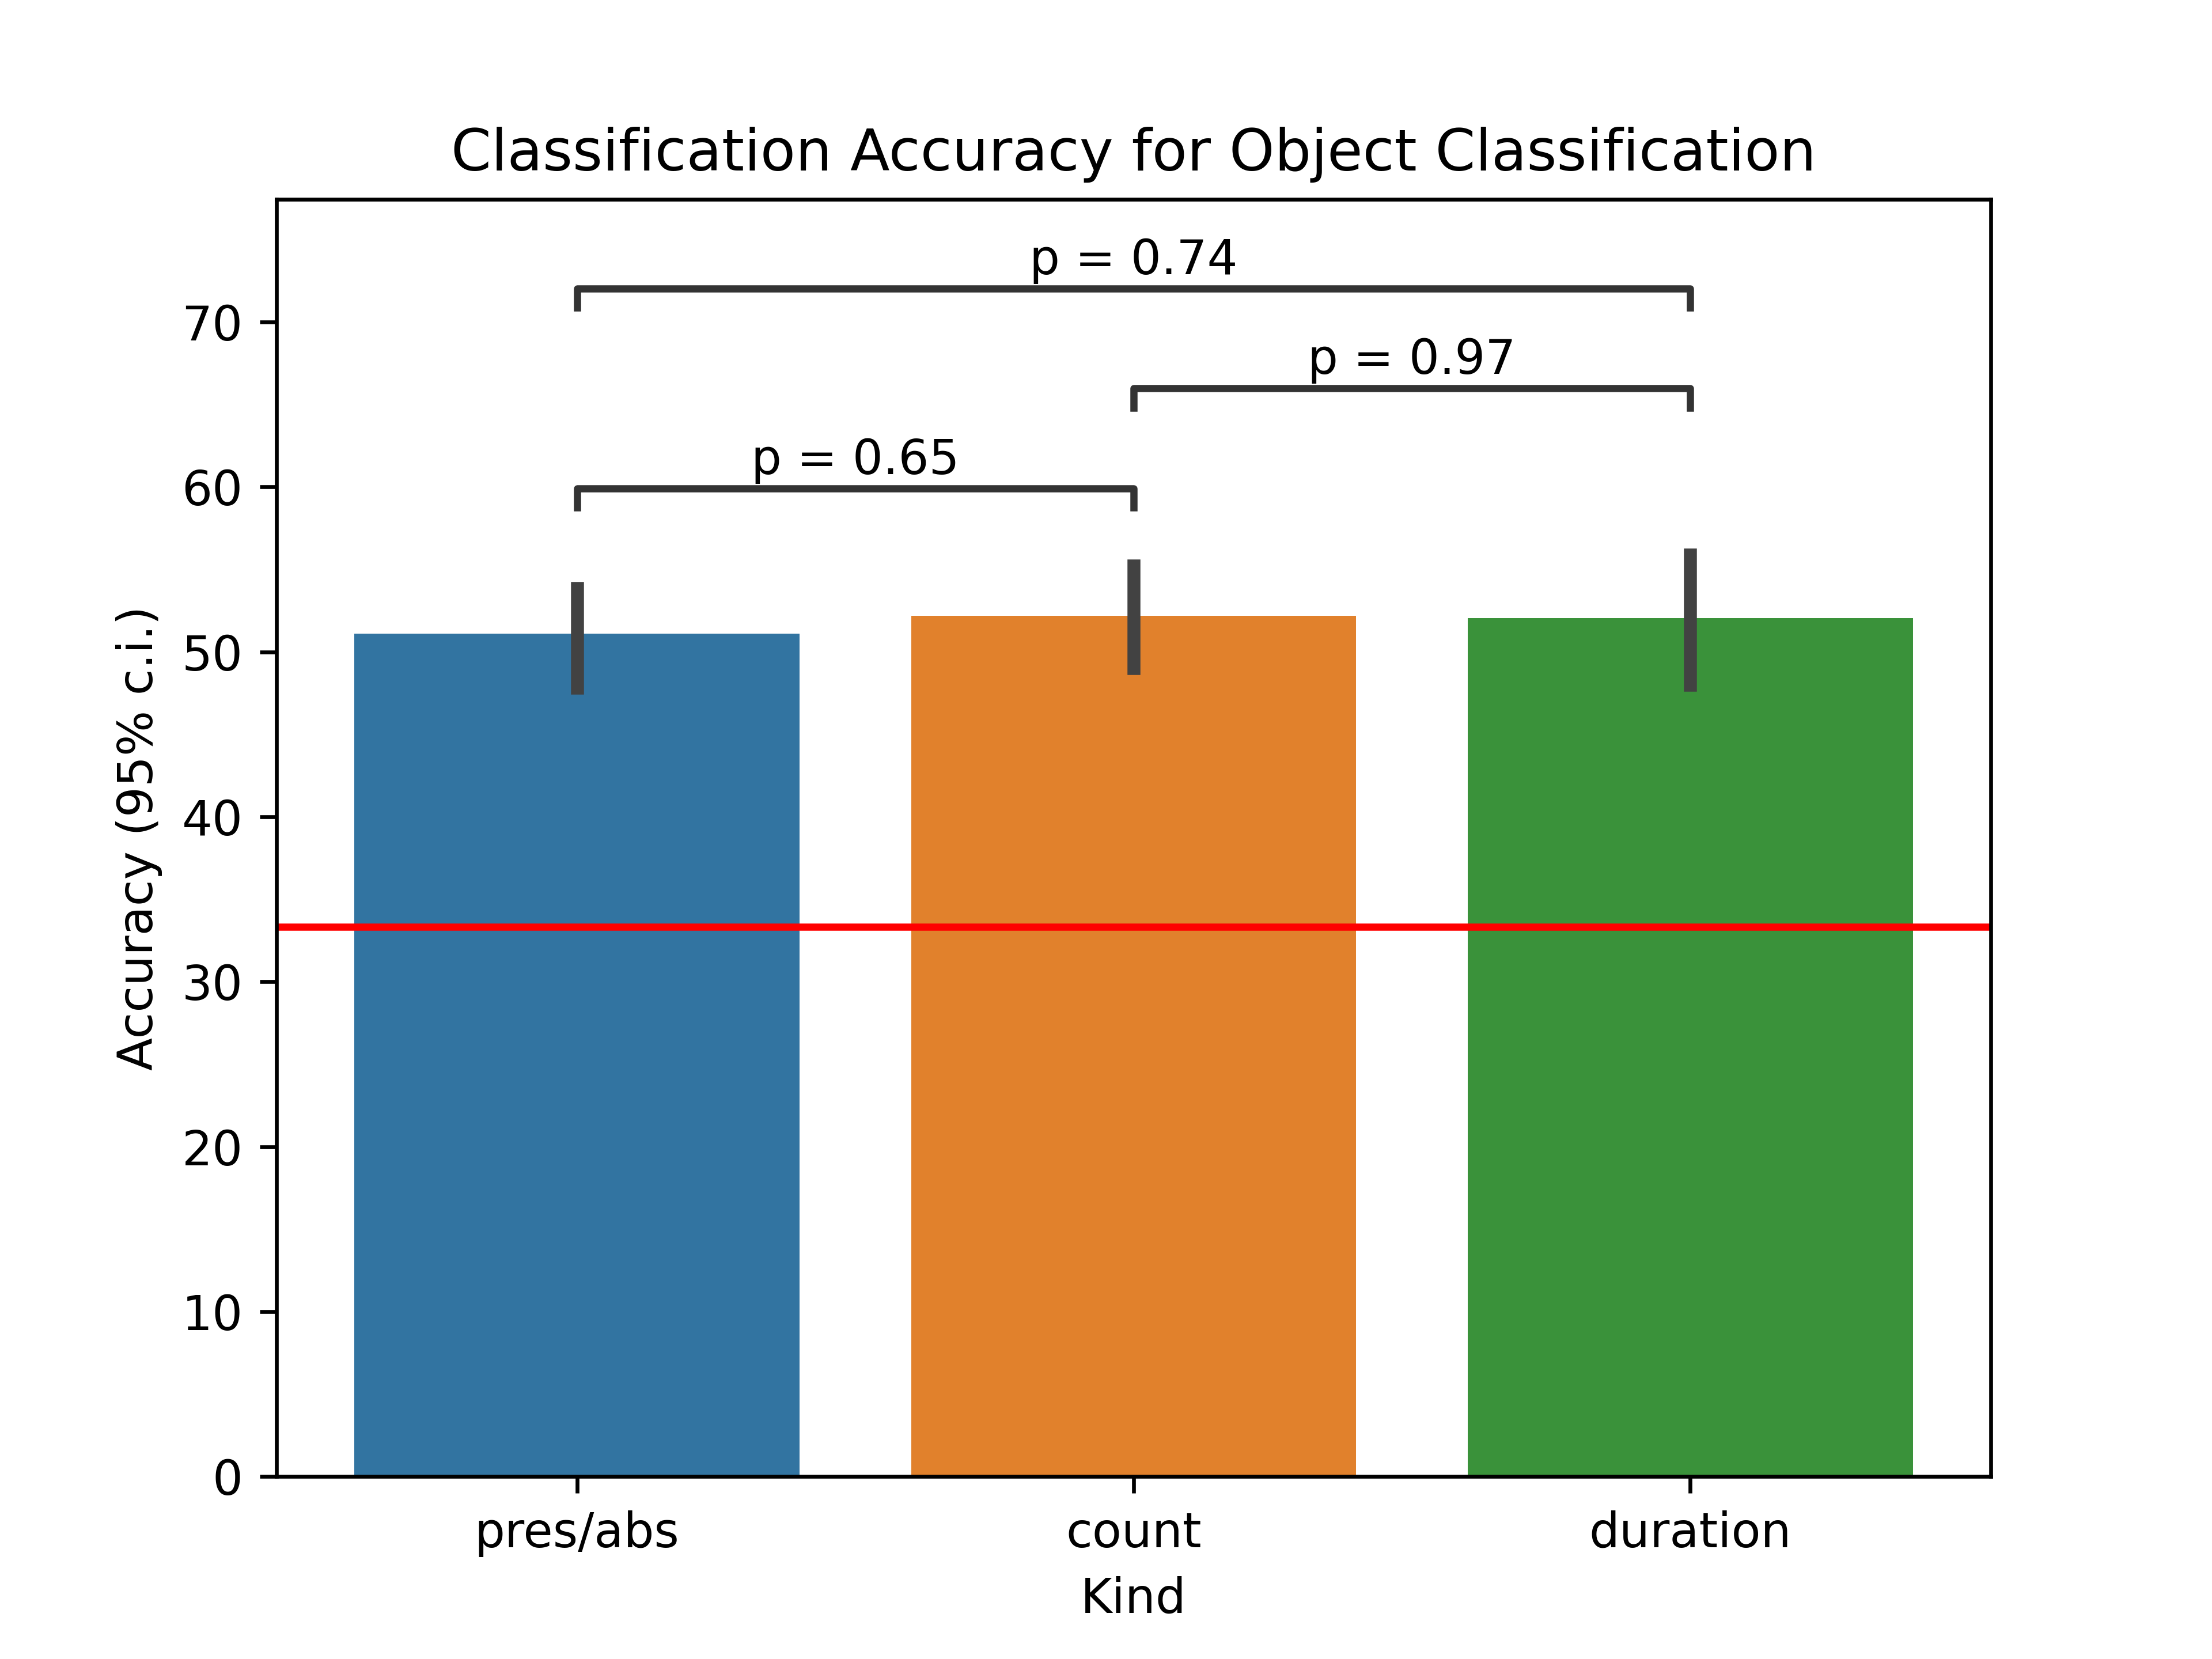
\includegraphics[width=0.75\textwidth]{./figures/EP_obj_class_acc.png}
\caption{Classification accuracy for object classification (given object)}
\label{ep_giv_obj_class_acc}
\end{centering}
\end{figure} 

\subsubsection*{Asked Object Classification}

Since it remains unclear that the classification of given object is really informative, we have tried also classification of \textbf{asked object}.

\begin{figure}[!h]
\begin{centering}
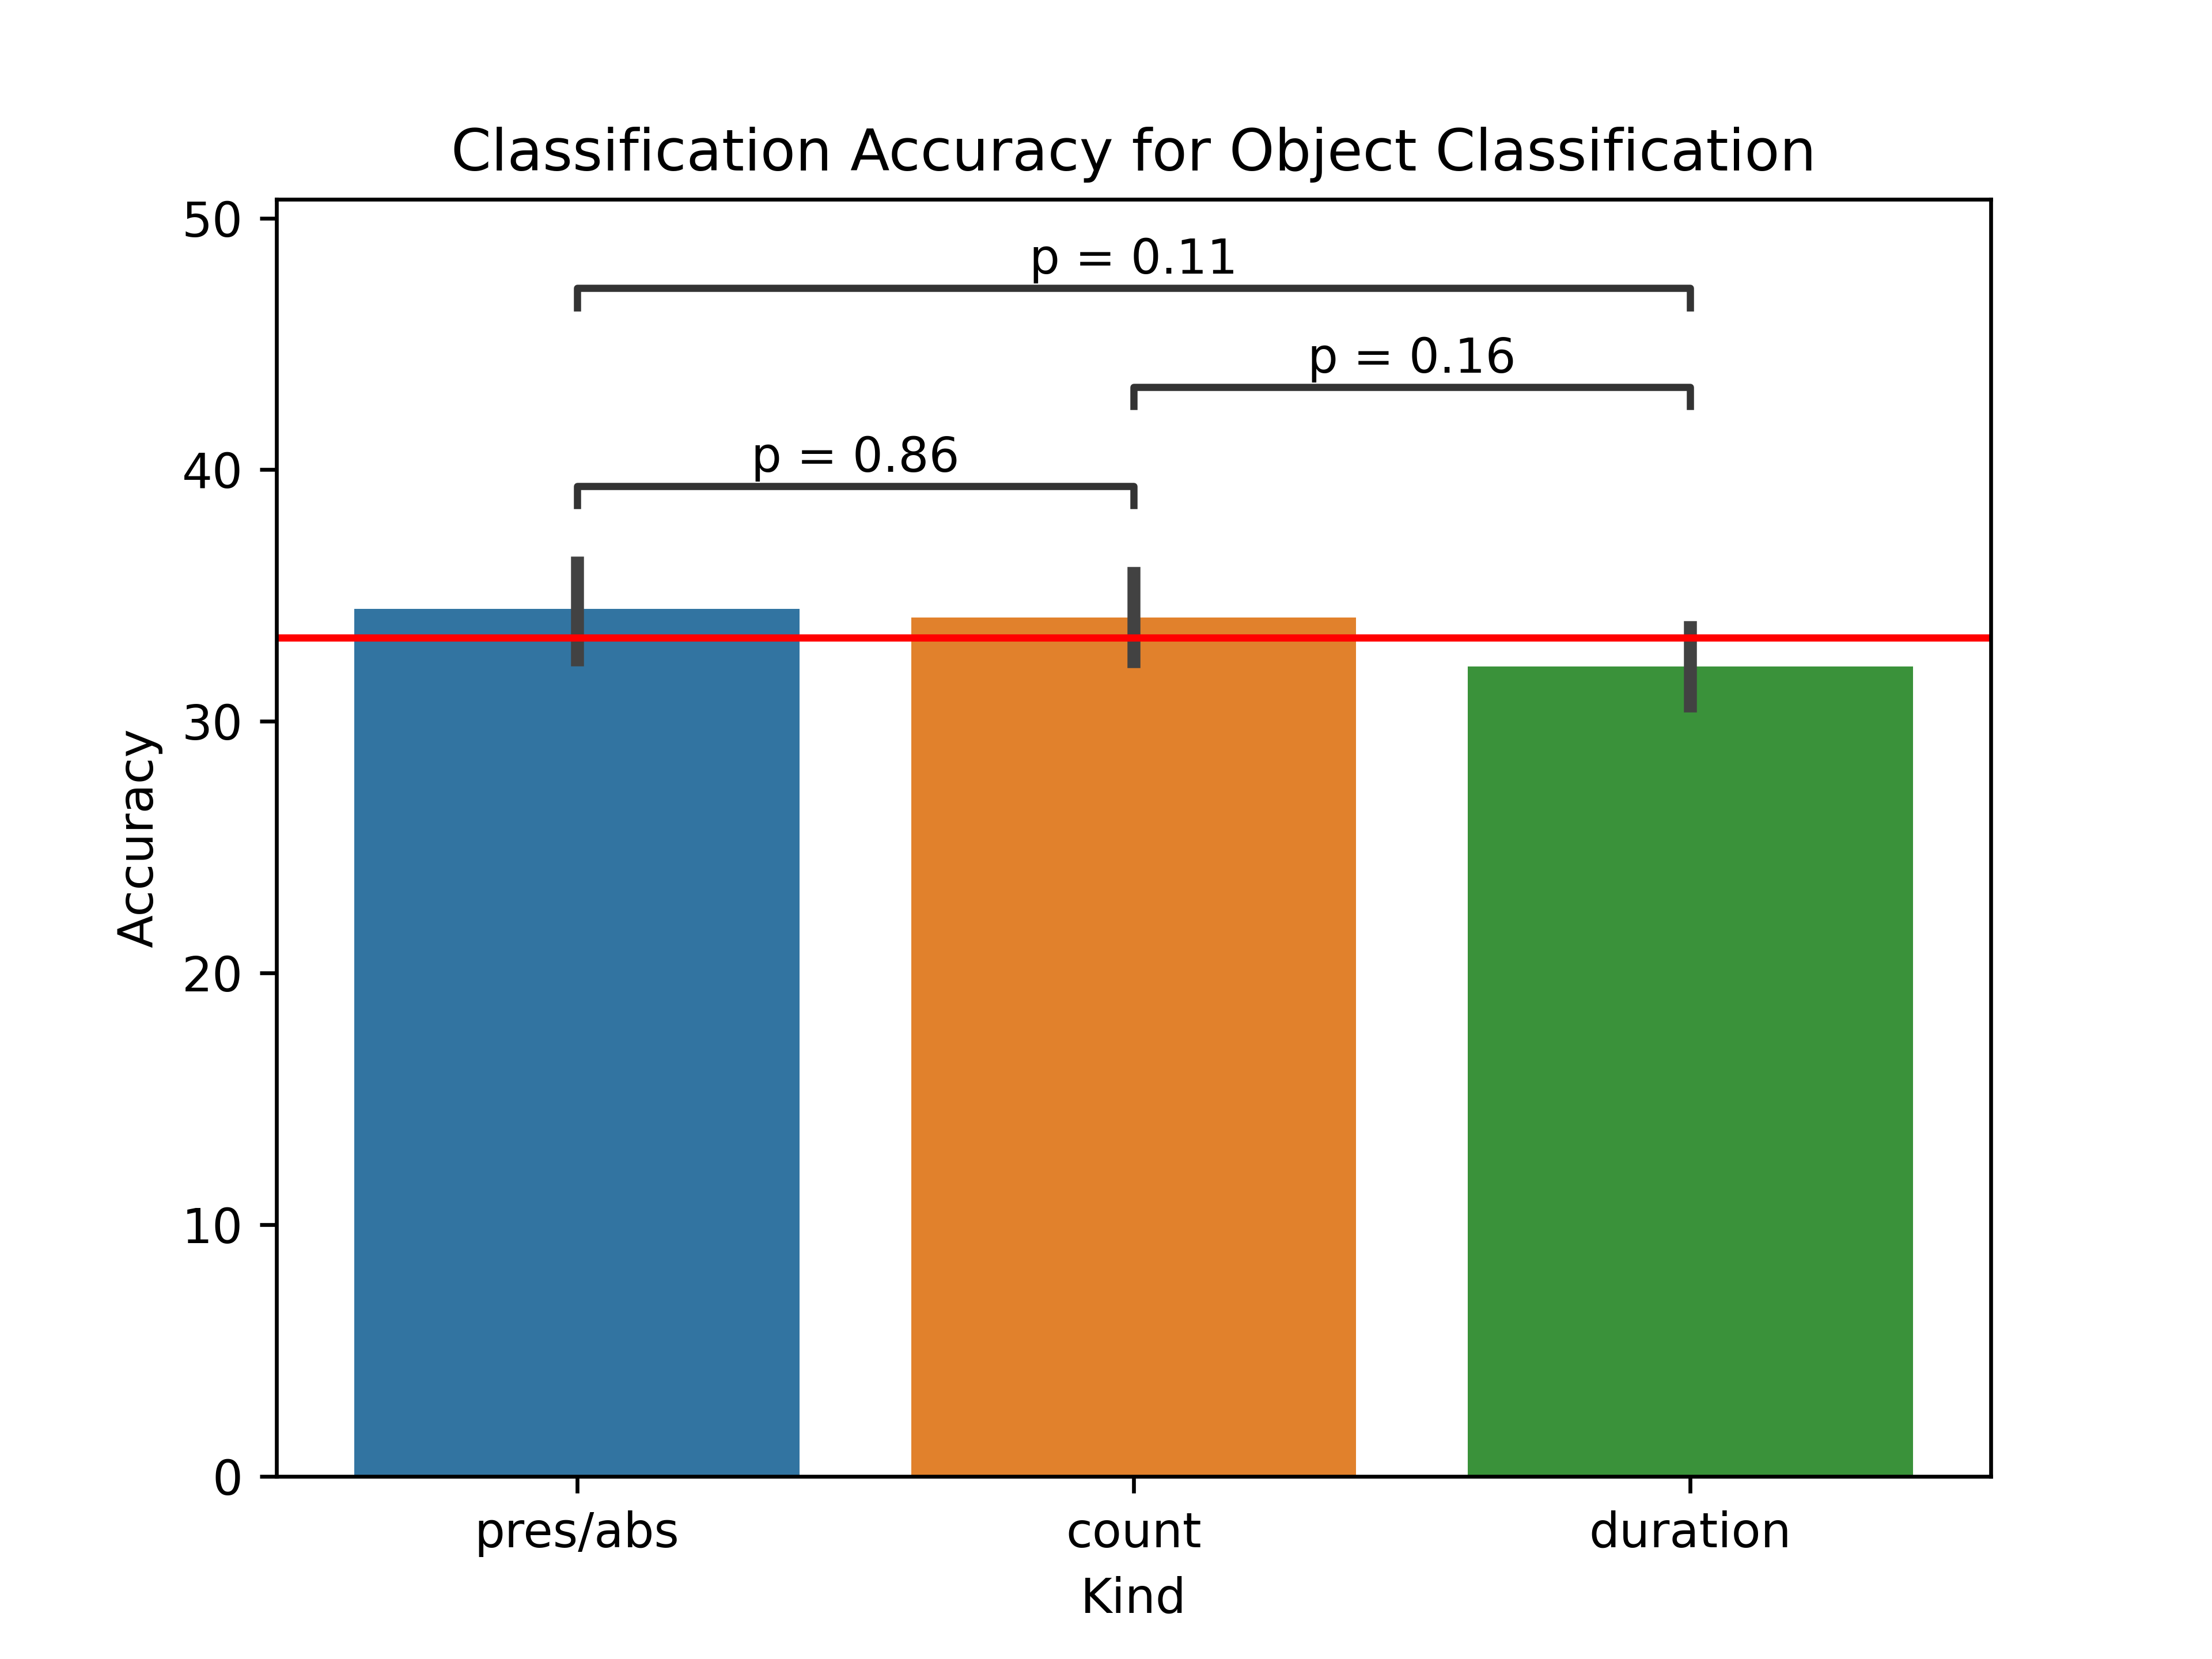
\includegraphics[width=0.75\textwidth]{./figures/giv_EP_obj_class_acc.png}
\caption{Classification accuracy for object classification (asked object)}
\label{ep_ask_obj_class_acc}
\end{centering}
\end{figure}

\paragraph{}
As we can see in Figure \ref{ep_ask_obj_class_acc}, the accuracy in this case is near chance level. 

\subsubsection*{Object Classification conclussions}
Since the classification is within group, this results show how good are EPs to distinguish between objects inside the same group. We can conclude in this case that the EPs performed are somehow related to the object that subject is handling and not at all related with the object that we are asking for. 

\subsection*{Family Classification}
In this case, we want to predict the family to which the provided object belongs. 

\begin{figure}[!h]
\begin{centering}
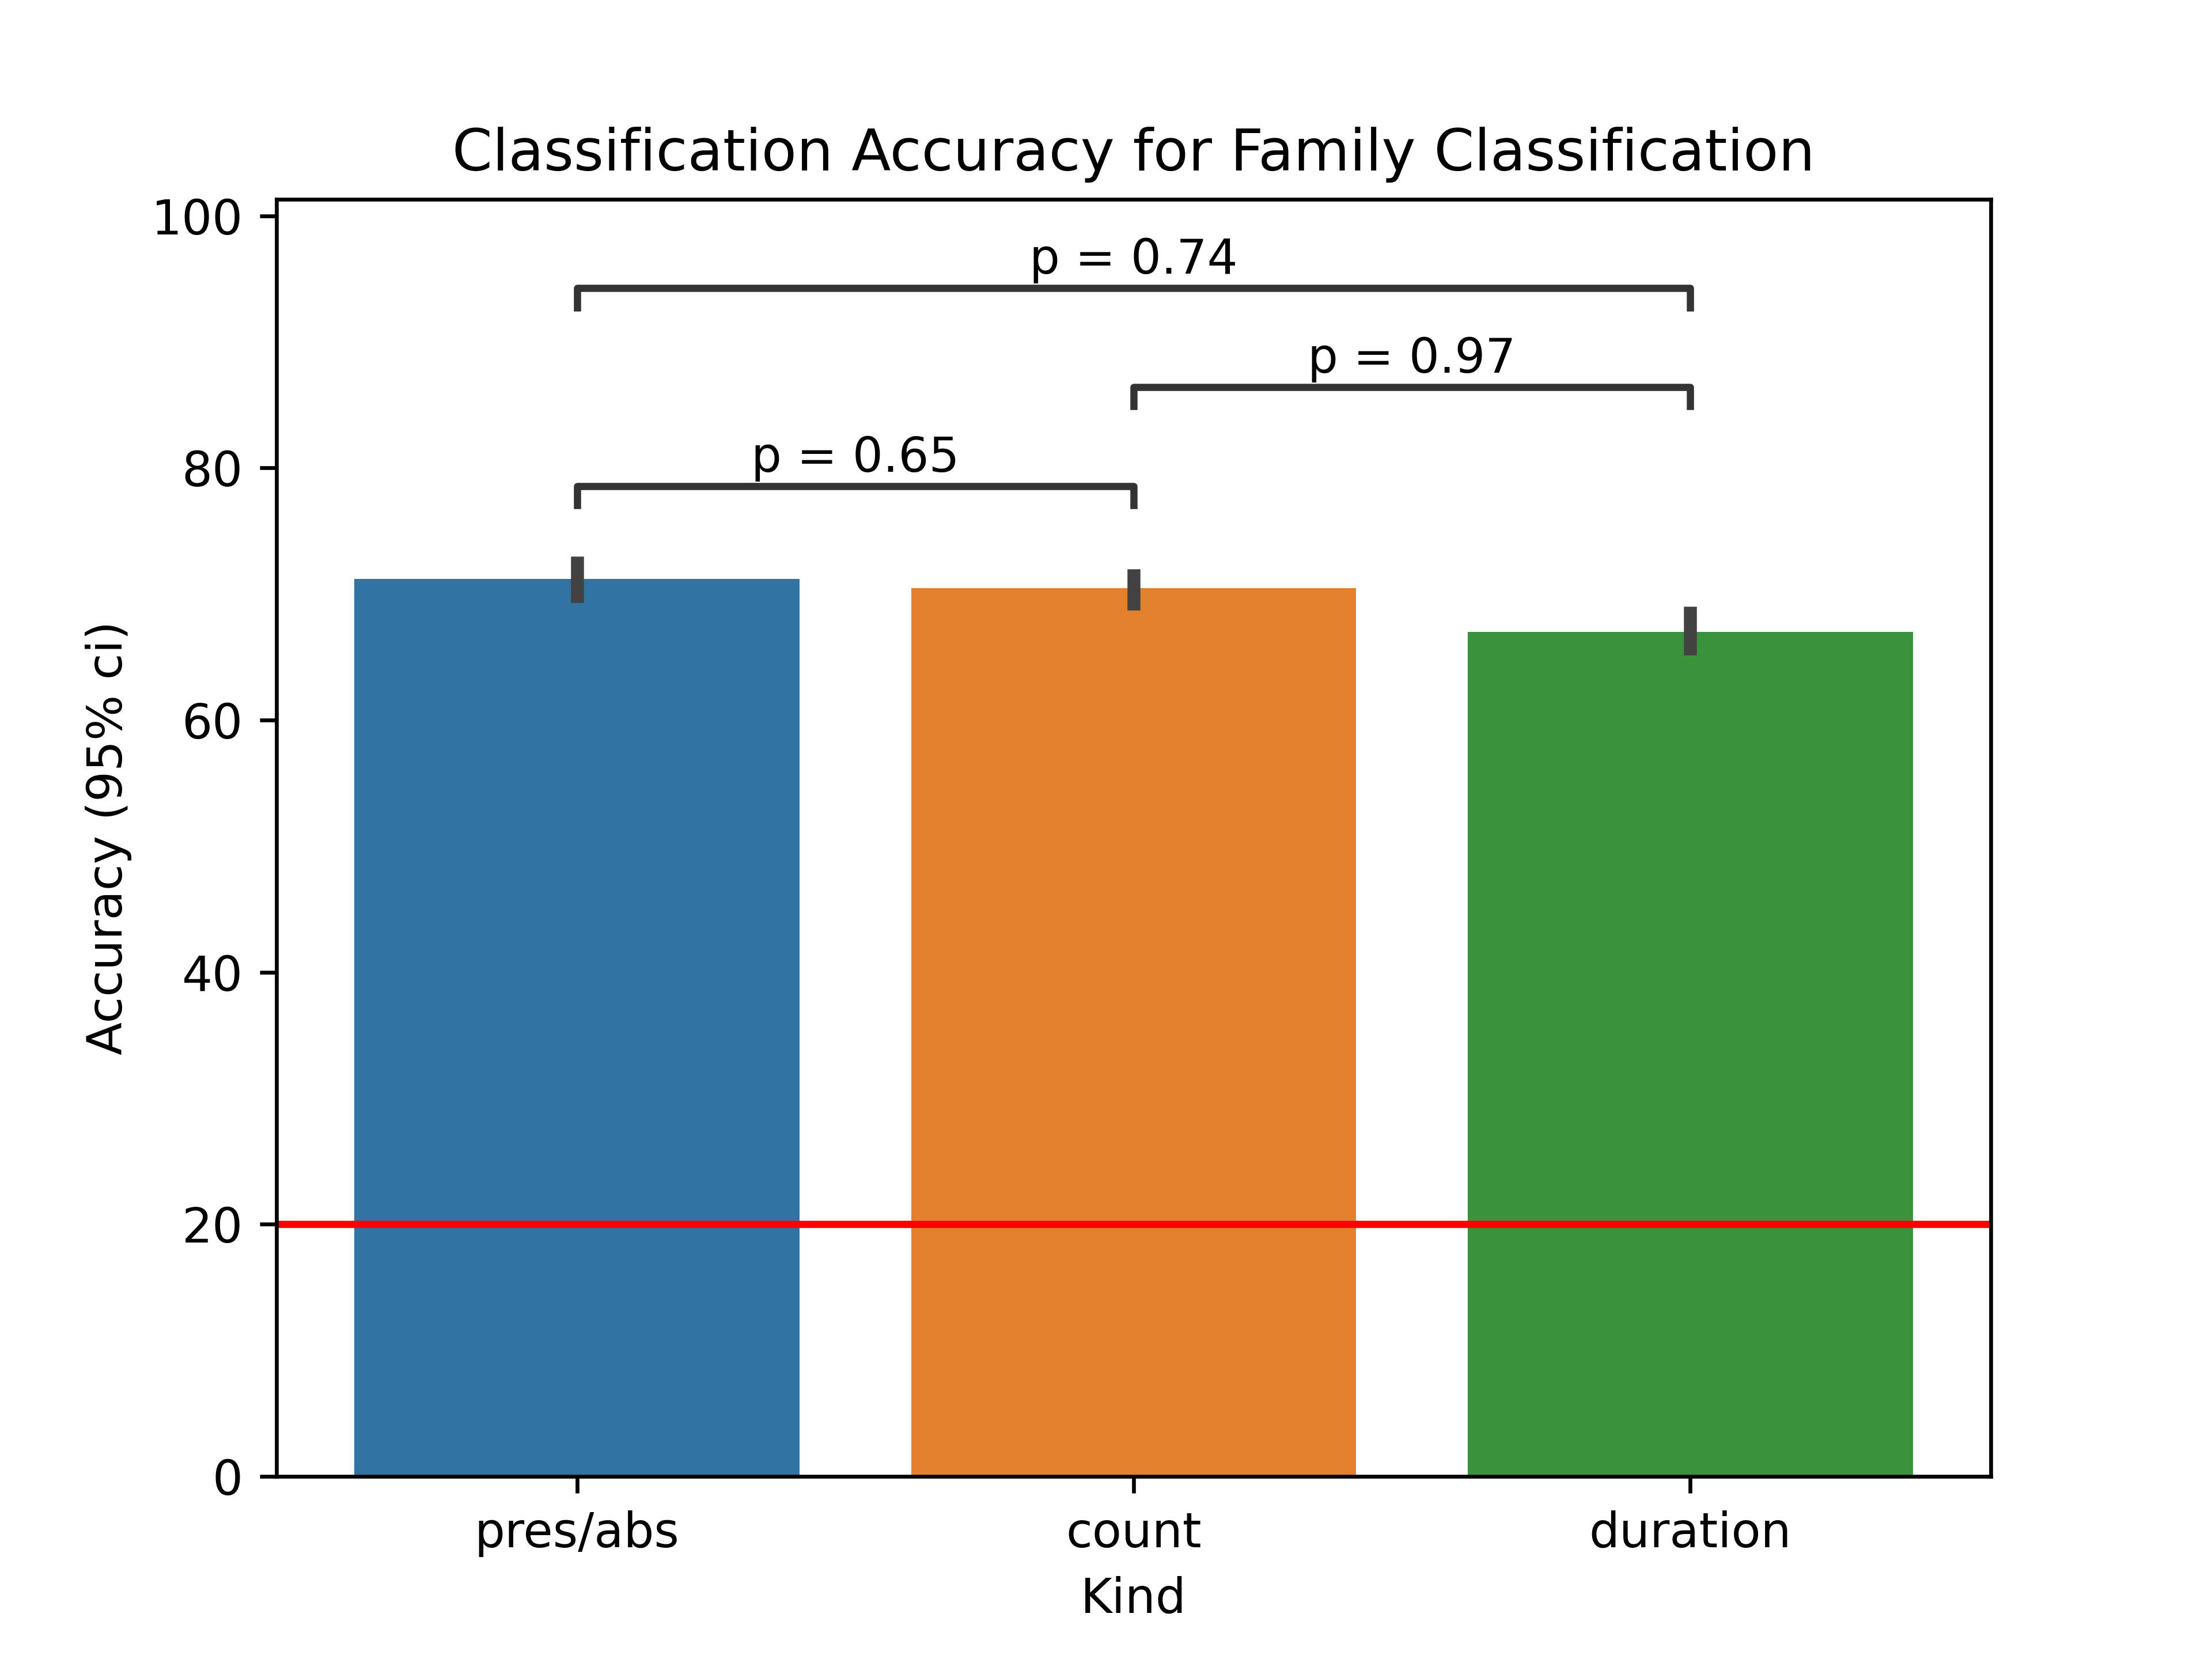
\includegraphics[width=0.75\textwidth]{./figures/EP_fam_class_acc.png}
\caption{Classification accuracy for family classification}
\label{ep_fam_class_acc}
\end{centering}
\end{figure}

\paragraph{}
Figure \ref{ep_fam_class_acc} shows a high accuracy for all three classifiers to predict the family.

\end{document}
